%\listfiles
\documentclass[tg]{mdtufsm}
% um tipo específico de monografia pode ser informado como parâmetro opcional:
%\documentclass[tese]{mdtufsm}
% a opção `openright' pode ser usada para forçar inícios de capítulos
% em páginas ímpares
% \documentclass[openright]{mdtufsm}
% para gerar uma versão frente-e-verso, use a opção 'twoside':
% \documentclass[twoside]{mdtufsm}

\usepackage[T1]{fontenc}        % pacote para conj. de caracteres correto
\usepackage{fix-cm} %para funcionar corretamente o tamanho das fontes da capa
\usepackage{times, color, xcolor}       % pacote para usar fonte Adobe Times e cores
\usepackage[utf8]{inputenc}   % pacote para acentuação
\usepackage{graphicx}  % pacote para importar figuras
\usepackage{amsmath,latexsym,amssymb} %Pacotes matemáticos
\usepackage[%hidelinks%, 
            bookmarksopen=true,linktoc=none,colorlinks=true,
            linkcolor=black,citecolor=black,filecolor=magenta,urlcolor=blue,
            pdftitle={Título da Dissertação ou Trabalho ....},
            pdfauthor={Nome Autor Sobrenome},
            pdfsubject={Dissertação de Mestrado},
            pdfkeywords={Dissertação, Modelo, LaTeX}
            ]{hyperref} %hidelinks disponível no pacote hyperref a partir da versão 2011-02-05  6.82a
%Nesse caso, hidelinks retira os retângulos em volta dos links das referências

%Margens conforme MDT 7ª edição, arrumar diretamente no mdtufsm.cls para funcionar a opção twoside *PENDENTE*
\usepackage[inner=30mm,outer=20mm,top=30mm,bottom=20mm]{geometry} 
\usepackage{array}
\usepackage{float}
\usepackage{listings}


%==============================================================================
% Se o pacote hyperref foi carregado a linha abaixo corrige um bug na hora
% de montar o sumário da lista de figuras e tabelas
% Se o pacote não foi carregado, comentar a linha %
%==============================================================================

%%=============================================================================
%% Trampa para corrigir o bug do hyperref que redefine o caption das figuras e das
%% tabelas, n�o colocando o nome ``Figura'' antes do n�mero do mesmo na lista
%%=============================================================================

\makeatletter

\long\def\@caption#1[#2]#3{%
  \expandafter\ifx\csname if@capstart\expandafter\endcsname
                  \csname iftrue\endcsname
    \global\let\@currentHref\hc@currentHref
  \else
    \hyper@makecurrent{\@captype}%
  \fi
  \@ifundefined{NR@gettitle}{%
    \def\@currentlabelname{#2}%
  }{%
    \NR@gettitle{#2}%
  }%
  \par\addcontentsline{\csname ext@#1\endcsname}{#1}{%
    \protect\numberline{\csname fnum@#1\endcsname ~-- }{\ignorespaces #2}%
  }%
  \begingroup
    \@parboxrestore
    \if@minipage
      \@setminipage
    \fi
    \normalsize
    \expandafter\ifx\csname if@capstart\expandafter\endcsname
                    \csname iftrue\endcsname
      \global\@capstartfalse
      \@makecaption{\csname fnum@#1\endcsname}{\ignorespaces#3}%
    \else
      \@makecaption{\csname fnum@#1\endcsname}{%
        \ignorespaces
        \ifHy@nesting
          \expandafter\hyper@@anchor\expandafter{\@currentHref}{#3}%
        \else
          \Hy@raisedlink{%
            \expandafter\hyper@@anchor\expandafter{%
              \@currentHref
            }{\relax}%
          }%
          #3%
        \fi
      }%
    \fi
    \par
  \endgroup
}

\makeatother

%==============================================================================
% Identificação do trabalho
%==============================================================================
\title{Ferramenta Computacional para Síntese de Filtros Analógicos e Digitais}

\author{Pinheiro}{Renan Birck}
%Descomentar se for uma "autora"
%\autoratrue

\course{Graduação no curso de Engenharia Elétrica}
\altcourse{curso de Engenharia Elétrica}

\institute{Centro de Tecnologia}
\degree{Engenheiro Eletricista}

% Número do TG (verificar na secretaria do curso)
% Para mestrado deixar sem opção dentro do {}
\trabalhoNumero{}

%Orientador
\advisor[Prof.]{Dr.}{de Tal}{Fulano}
%Se for uma ``orientadora'' descomentar a linha baixo
%\orientadoratrue

%Co orientador, comentar se não existir
%\coadvisor[Prof.]{Drª.}{Pereira}{Maria Regina}
%\coorientadoratrue %Se for uma ``Co-Orientadora''

%Avaliadores (Banca)
\committee[Dr.]{De Tal}{Fulano}{UFSM}
\committee[Dr.]{De Tal}{Sicrano}{UFSM}

% a data deve ser a da defesa; se nao especificada, são gerados
% mes e ano correntes
\date{XX}{junho}{2015}

%Palavras chave
\keyword{Filtros eletrônicos} 
\keyword{Ferramenta computacional}
\keyword{Projeto Eletrônico}


%%=============================================================================
%% Início do documento
%%=============================================================================
\begin{document}

%%=============================================================================
%% Capa e folha de rosto
%%=============================================================================
\maketitle

%%=============================================================================
%% Catalogação (obrigatório para mestrado) e Folha de aprovação
%%=============================================================================
%Somente obrigatório para dissertação, para TG, remover as linhas	77	%
%Como a CIP vai ser impressa atrás da página de rosto, as margens inner e outer	
%devem ser invertidas.
\newgeometry{inner=20mm,outer=30mm,top=30mm,bottom=20mm}	
\makeCIP{renan.ee.ufsm@gmail.com} %email do autor		
\restoregeometry

%Se for usar a catalogação gerada pelo gerador do site da biblioteca comentar as linhas
%acima e utilizar o comando abaixo
%\includeCIP{CIP.pdf}

%folha de aprovação
\makeapprove

%%=============================================================================
%% Dedicatória (opcional)
%%=============================================================================
%\clearpage
%\begin{flushright}
%\mbox{}\vfill
%{\sffamily\itshape À UFSM ......}
%\end{flushright}

%%=============================================================================
%% Agradecimentos (opcional)
%%=============================================================================
\chapter*{Agradecimentos}
À minha família e amigos pelo apoio e incentivo durante minha trajetória no curso.

Ao professor Fulano de Tal, por ter me orientado na execução deste trabalho.

Aos meus colegas de trabalho na Chip Inside Tecnologia, que colaboraram na revisão deste trabalho e sugeriram correções e modificações.

%%=============================================================================
%% Epígrafe (opcional)
%%=============================================================================
\clearpage
\begin{flushright}
\mbox{}\vfill
{\sffamily\itshape
``Se o Pica-Pau tivesse comunicado à polícia, isso nunca teria acontecido.'' \\ }
--- \textsc{Anônimo}
\end{flushright}


%%=============================================================================
%% Resumo
%%=============================================================================
\begin{abstract}
Blá blá blá.
\end{abstract}

%%=============================================================================
%% Abstract
%%=============================================================================
% resumo na outra língua
% como parametros devem ser passados o titulo, o nome do curso,
% as palavras-chave na outra língua, separadas por vírgulas, o mês em inglês
%o a sigla do dia em inglês: st, nd, th ...
\begin{englishabstract}
{Development of a Software Tool for Analog and Digital Filter Design}
{Electrical Engineer}
{Foo, Bar, Baz}
{January}
{st}

This work\dots
\end{englishabstract}

%% Lista de Ilustrações (opc)
%% Lista de Símbolos (opc)
%% Lista de Anexos e Apêndices (opc)

%%=============================================================================
%% Lista de figuras (comentar se não houver)
%%=============================================================================
\listoffigures

%%=============================================================================
%% Lista de tabelas (comentar se não houver)
%%=============================================================================
\listoftables

%%=============================================================================
%% Lista de Apêndices (comentar se não houver)
%%=============================================================================
%\listofappendix

%%=============================================================================
%% Lista de Anexos (comentar se não houver)
%%=============================================================================
\listofannex

%%=============================================================================
%% Lista de abreviaturas e siglas
%%=============================================================================
 %o parametro deve ser a abreviatura mais longa
\begin{listofabbrv}{UbiComp}
\item [DSP] \textit{Digital Signal Processing}
\item[FFT] \textit{Fast Fourier Transform}
\end{listofabbrv}


%%=============================================================================
%% Lista de simbolos (opcional)
%%=============================================================================
%Simbolos devem aparecer conforme a ordem em que aparecem no texto
% o parametro deve ser o símbolo mais longo
%\begin{listofsymbols}{teste}
%  \item [$\varnothing$] vazio
%  \item [$\Gamma$]  Gama
%  \item [$\forall$] Para todo
%\end{listofsymbols}

%%=============================================================================
%% Sumário
%%=============================================================================
\tableofcontents


%%=============================================================================
%% Início da dissertação
%%=============================================================================
\setlength{\baselineskip}{1.5\baselineskip}

%Adiciona cada capitulo
\chapter{Introdução}

Blá blá blá.

\section{Motivação}
As seguintes razões motivaram a escolha do tema e a escrita deste trabalho:
\begin{itemize}
\item Blá
\item Blá
\item Blá
\end{itemize}

\section{Objetivos}

Os objetivos principais deste trabalho são:

\begin{itemize}
\item Blá
\item Blá
\item Blá 
\end{itemize}


\section{Estrutura do trabalho}

O capítulo 2 irá realizar uma revisão teórica dos conhecimentos empregados nesse trabalho. No capítulo 3 será abordado o processo de desenvolvimento, seguindo-se um capítulo no qual o \textit{software} desenvolvido será demonstrado e discutido. Após, serão apresentadas conclusões e sugestões para futuras melhorias.

\chapter{Fundamentação Teórica}

Neste capítulo  serão apresentados as informações adquiridas através de pesquisas em diversas fontes, bem como os conhecimentos obtidos durante o curso de Engenharia de Computação os quais tornaram possível a implementação deste trabalho. Primeiramente será comentado sobre o funcionamento e os componentes de um chuveiro convencional e após será discutido informações sobre os dispositivos e componentes utilizados no presente trabalho.

\section{Funcionamento de um chuveiro elétrico}

O funcionamento de um chuveiro elétrico, independente do modelo ou marca, é praticamente o mesmo, na maioria dos modelos. Ao abrir o registro a água irá passar pelo diafragma pressionando-o para que haja contato entre dois terminais possibilitando assim o fornecimento de energia elétrica para o chuveiro. Com o contato feito, a corrente elétrica passa pela resistência do chuveiro esquentando-a e consequentemente esquentando a água. Este mecanismo impede que haja passagem de corrente elétrica na resistência do chuveiro caso o registro seja fechado, o que ocasionaria um superaquecimento e o comprometimento do funcionamento do chuveiro. Este fenômeno que transforma energia elétrica em energia térmica é denominado efeito Joule.

\subsection{Componentes de um chuveiro}

Os componentes principais de um chuveiro elétrico, para seu funcionamento correto são o espalhador, o diafragma e a resistência elétrica. Em duchas eletrônicas existe o componente interno chamado TRIAC do qual seu funcionamento também será comentado no presente trabalho.

\subsection{Resistência}

A resistência elétrica de um chuveiro é composta de um fio de Nicromo (material condutor constituído de Niquel e Cobre) enrolado. A corrente elétrica passa por este material e, desta forma, aquece a água para o banho. A figura 2.1 mostra um exemplo de uma resistência elétrica.

\begin{figure}[h]

\center

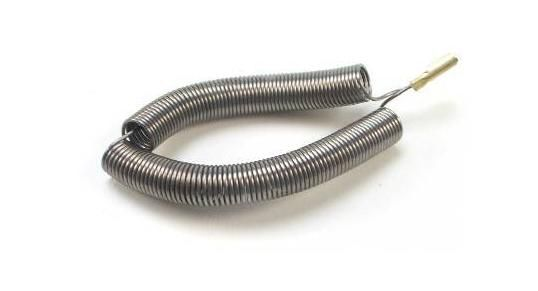
\includegraphics[width=10cm]{imagens/resistencia.jpg}

\label{Resistência de um chuveiro}

\caption{Resistência de um chuveiro}

\end{figure}

\subsection{Diafragma}

O diafragma é um componente que funciona como uma chave para a alimentação do chuveiro. Quando o registro é aberto, a água ao passar pelo chuveiro pressiona o diafragma fazendo com que dois pontos entrem em contato conectando o chuveiro a rede elétrica e, dessa forma, tem-se corrente elétrica circulando pela resistência. Ele é uma peça crucial, pois ao desligar-se o chuveiro a tensão no chuveiro é cortada e assim não há mais passagem de corrente elétrica na resistência evitando acidentes devido ao superaquecimento da resistência elétrica.A figura 2.2 ilustra o funcionamento de um diafragma.

\begin{figure}[!htb]

\center

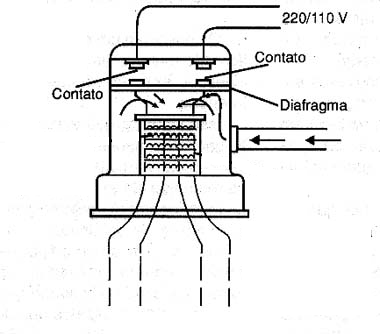
\includegraphics[width=5cm]{imagens/diafragma.png}

\label{Diafragma}

\caption{Diafragma}

\end{figure}

\subsection{Espalhador}

O espalhador é um elemento do chuveiro onde há a saída da água aquecida pela resistência. Ele possui pequenos orifícios que dificultam a passagem da água, funcionando como um limitador de vazão e fazendo com que o diafragma fique pressionado mantendo dois pontos em contato para que haja passagem de corrente elétrica.A figura 2.3 mostra o espalhador de um chuveiro convencional.


\begin{figure}[!htb]

\center

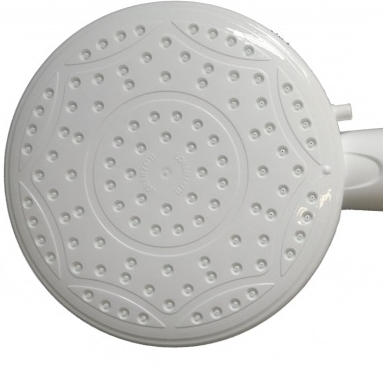
\includegraphics[width=7cm]{imagens/espalhador.png}

\label{Espalhador}

\caption{Espalhador}

\end{figure}


\section{Microcontrolador}

Um microcontrolador é um dispositivo presente em inúmeros aparelhos eletrônicos do dia-a-dia, como celulares, microondas, geladeiras, dentre outros. Ele é constiuído de um processador, memória de programa, memória de dados, pinos de \textit{I/O} (\textit{Input/Output}) e mais alguns periféricos como \textit{timers}, conversores A/D (analógico/digitais), dentre outros, tudo em apenas um encapsulamento, tornando assim menor a complexidade do circuito eletrônico que seria utilizado para uma determinada aplicação de controle.  Por esse motivo, os microcontroladores são ótimas ferramentas para a implementação de projetos de sistemas embarcados,onde há necessidade de um controle específico e regulado.


\subsection{Arduino}
O Arduino Uno (Uno, 2013) é uma plataforma de prototipagem eletrônica gratuita que utiliza um microcontrolador da família ATmega de 8 \textit{bits}. Ele é capaz de trabalhar com inúmeros tipos de aplicações como sensores, motores, \textit{leds}, dentre outros. No presente trabalho foi utilizado o modelo do Arduino chamado UNO que utiliza o microcontrolador ATmega328.

\begin{figure}[h]

\center

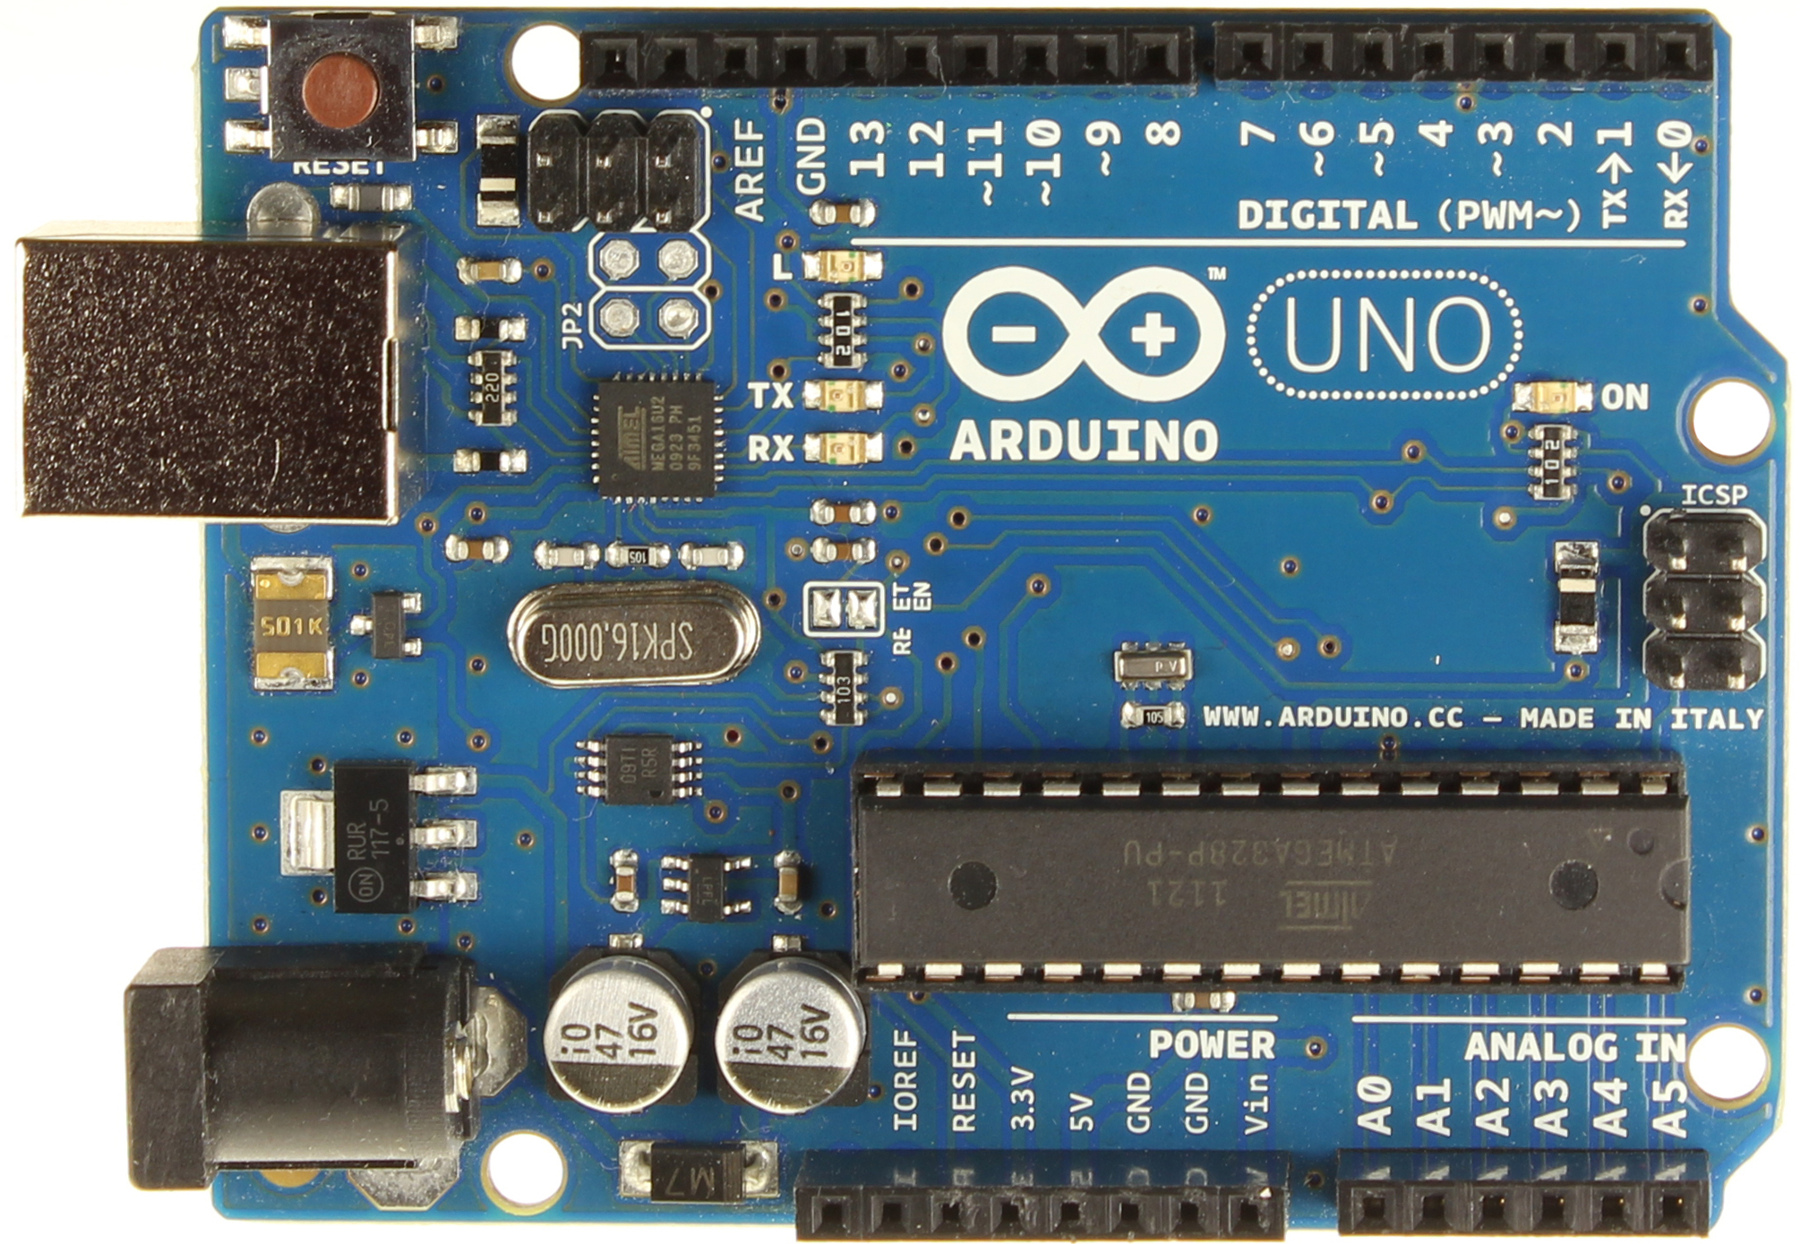
\includegraphics[width=10cm]{imagens/arduino_uno.jpg}

\label{Arduino UNO}

\caption{Arduino UNO}

\end{figure}

\subsection{ATmega328}
O ATmega328 é um microcontrolador, pertencente à família AVR da empresa ATmel que é utilizado no Arduino UNO. Este modelo de microcontrolador possui um processador RISC (\textit{Reduced Instruction Set Computing}) de 8 bits que utiliza uma arquitetura Harvard modificada, possui 32KB de memória flash, 1KB de EEPROM (\textit{Electrically-Erasable ProgrammableRead-Only Memory}), 2KB de SRAM (\textit{Static Random Access Memory}), 32 registradores, três \textit{timers} (temporizadores), uma USART (\textit{Universal Synchronous Asynchronous Receiver Transmitter}), portas para comunicação SPI (\textit{Serial Peripheral Interface}), um conversor AD de 10 bits, saídas PWM (\textit{Pulse-Width Modulation}) dentre outros(ATmega328 Datasheet, 2009). O ATmega328 é utilizado em alguns modelos de Arduino encontrados no mercado. Na tabela 2.1 são mostrados alguns dados do microcontrolador fornecidos pelo fabricante.

\begin{table}[!hbt] 
   \centering   % tabela centralizada
   \setlength{\arrayrulewidth}{1\arrayrulewidth}
   \setlength{\belowcaptionskip}{5pt}
   
   \caption{Caracteristicas do Arduino UNO}
   \begin{tabular}{l|l} % c=center, l=left, r=right 
      \hline
      Microcontrolador & ATmega328 \\
      \hline
      Tensão de operação & 5V  \\
      \hline
      Tensão de entrada (recomendado)  & 7-12V \\
      \hline
      Pinos digitais de I/O	& 14 (6 com saída PWM) \\
      \hline
      Pinos de entrada analógica &	6\\
      \hline
      Corrente por pino de I/O &	40 mA\\
      \hline
      Corrente pelo pino de 3,3V&	50 mA\\
      \hline
      Memória Flash & 32KB (ATmega328)\\
      \hline
      SRAM & 2 KB (ATmega328)\\
      \hline
      EEPROM & 1KB (ATmega328)\\
      \hline
      Velocidade do Clock & 16 MHz\\
   \end{tabular}
   \label{Características do Arduino UNO}
\end{table}

O Arduino possui uma IDE (\textit{Integrated Development Environment}) que é uma aplicação escrita em linguagem java onde pode-se desenvolver códigos em linguagem C/C++ para controlar os pinos do microcontrolador. Esta IDE está disponível para download gratuitamente no site do fornecedor (Arduino,2013).



\subsubsection{Pinagem}
O microcontrolador ATmega328 possui, ao total, 28 pinos dos quais são divididos da seguinte forma:

\begin{itemize}
\item	14 pinos digitais de entrada e saída (configuráveis).
\item	6 pinos de entrada analógica ou entrada e saída digital     (configuráveis).
\item	5 pinos de alimentação (terra, 5V, referência analógica).
\item	1 pino de reset.
 \item   2 pinos para conexão de um cristal oscilador.
\end{itemize}

\begin{figure}[h]

\center

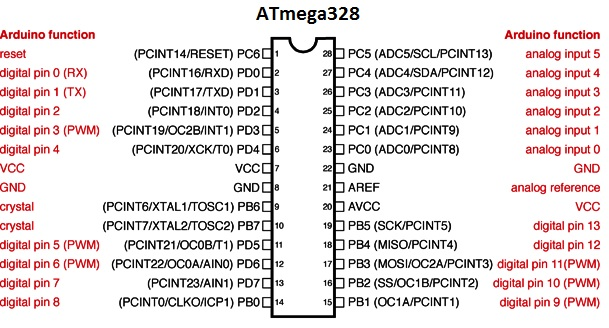
\includegraphics[width=10cm]{imagens/pinagematmega.jpg}

\label{Pinagem do ATmega328}

\caption{Pinagem do ATmega328}

\end{figure}
Os pinos digitais podem ser configurados como entrada ou saída e possuem somente dois estados: ligado (\textit{HIGH}) ou desligado(\textit{LOW}). Quando o pino é configurado como ligado ele apresenta uma tensão de saída de 5V e quando configurado como desligado apresenta na saída a tensão de zero Volts. Esses pinos podem ser utilizados para várias aplicações como acendimento de \textit{leds}, operações com portas lógicas, acionamento de relés, dentre outros.

Os pinos analógicos são utilizados na maioria das vezes para leituras de sensores e transdutores que convertem grandezas físicas em tensão elétrica, a qual pode ser medida pela entrada analógica no microcontrolador.

\subsubsection{Pinos especiais}

Além dos pinos analógicos e digitais, o ATmega 328 possui uma quantidade de pinos com características especiais que podem ser configuradas através da programação. São eles:

\begin{itemize}
\item PWM (Pulse Width Modulation – Modulação por Largura de Pulso): é gerado um sinal pulsante, com uma determinada frequência, onde se define o tempo em que o sinal fica em nível alto e o tempo que o sinal fica em nível baixo. Desta forma, variando-se a razão cíclica, que é a razão entre tempo em nível alto e o período do sinal,  pode-se controlar o valor médio do sinal PWM. Os pinos que possuem saída PWM são: pinos 3,5,6,10 e 11. 

\item Portal Serial USART:  possibilita o microcontrolador se comunicar com um computador, bluetooth ou outro dispositivo do gênero, através de envio e recebimento de dados no formato serial assíncrono (USART). Os pinos que possuem comunicação serial são: pino 0 (recebe dados) e pino 1 (envia dados).

\item Interrupção externa: Existe a possibilidade de se programar um pino para que quando ativado force o processador a parar o que está fazendo e realizar outras operações pré-programadas. O ATmega328 possui 2 pinos (2 e 3) para interrupções externas. São bastante úteis para se economizar processamento em diversas aplicações.

\end{itemize}

\subsection{Vantagens}

As grandes vantagens de se utilizar a plataforma arduino são:
\begin{itemize}

\item	Ser uma ferramenta \textit{open-source} (\textit{Software/Hardware}).
\item	A gama de utilizadores da plataforma é grande, tendo assim uma grande quantidade de informações na rede, permitindo uma constante atualização sobre as inovações.
\item	Não tem a necessidade de operação em conjunto com um computador (\textit{Standalone}).
\item	Possibilidade de aumentar a capacidade de aplicações com a utilização de SHIELDS (placas de circuito impresso que podem ser plugadas ao pinos do microcontrolador possibilitando mais funções, como controlar motores e utilização de redes sem fio).

\end{itemize}

\subsection{Conversor A/D}

Um conversor A/D é um circuito que realiza a conversão de dados analógicos, de tensão ou corrente, para um valor digital com \textit{n bits}  Este circuito é bastante útil para diversos tipos de aplicações, como aquisição de dados de sensores, voz, áudio, entre outros.

O Arduino UNO possui pinos que utilizam um conversor A/D de 10 bits, ou seja, a tensão de referência é dividida por 1024 unidades ($2^{10}$). Por exemplo, suponha-se que a tensão de referência seja de 5V, teremos então 1024 valores entre a tensão de 0 à 5V, ou seja:

\begin{center}
Resolução $= 5V/1024 \approx 4,9mV$ 
\end{center}


Assim, a cada aumento de 4,9mV  na entrada do conversor A/D, tem-se o aumento de uma unidade digital.
\subsection{Comunicação serial}

A comunicação serial trata-se de um envio de forma sequencial de bits, por um barramento, em um certo intervalo de tempo, ou seja, de forma sequencial. Esse meio de comunicação é utilizado em diversos dispositivos como a USB (\textit{Universal Serial Bus}),\textit{FireWire}, RS-232 dentre outros. 

A Arduino UNO possui uma porta de comunicação nos pinos digitais 0 (recebimento de sinais digitais) e 1 (Envio de sinais digitais). A IDE do Arduino oferece uma aplicação bastante interessante e útil chamada de \textit{Serial Monitor} que quando utilizada mostra na tela os valores  das portas digitais e analógicas.

\begin{figure}[h]

\center

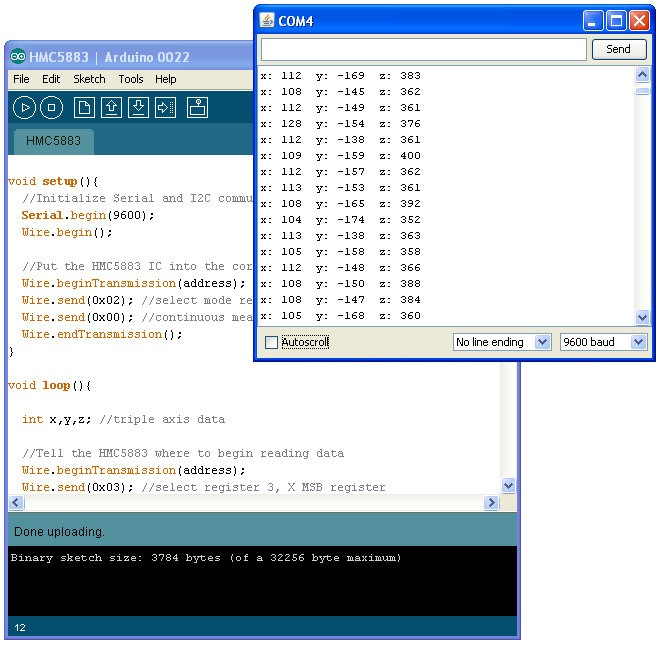
\includegraphics[width=10cm]{imagens/serial_monitor.jpg}

\label{Serial Monitor}

\caption{Serial Monitor}

\end{figure}

\subsection{Timers}

Os \textit{timers} são contadores internos do microcontrolador que podem ser limitados a um certo valor. A grande utilidade dos timers é de chamar uma determinada rotina num intervalo de tempo configurado (interrupção por tempo), como por exemplo realizar a leitura de um valor analógico em alguma porta do microcontrolador de 10 em 10 segundos.

Na tabela 2.2 são mostrados os timers do microcontrolador ATmega328 e suas características.

\begin{table}[!hbt] 
   \centering   % tabela centralizada
   \setlength{\arrayrulewidth}{1\arrayrulewidth}
   \setlength{\belowcaptionskip}{5pt}
   
   \caption{Timers do ATmega328}
   \begin{tabular}{l|l} % c=center, l=left, r=right 
   \hline
    Timer0 & temporizador de 8 bits que é utilizado nas funções          millis() e micros() \\
    \hline
    Timer1 & temporizador de 16 bits \\
    \hline
    Timer2 & temporizador de 8 bits\\
    \hline
   \end{tabular}
   \label{Timers do ATmega328}
\end{table}

\subsection{Interrupção}

Uma interrupção é um sinal do \textit{hardware} para mandar o processador suspender a tarefa que está executando no momento e executar outra determinada tarefa e,  após executada, o processador retornar a tarefa inicial sem a perda de informações(TANENBAUM, 1995).

O ATmega328 possui dois métodos diferentes de chamadas de interrupção: externa ou por tempo. A interrupção externa pode ser utilizada nos pinos digitais 2 e 3. A tabela 2.3 mostra os modos de chamada de interrupção que esses pinos utilizam.

\begin{table}[!hbt] 
   \centering   % tabela centralizada
   \setlength{\arrayrulewidth}{1\arrayrulewidth}
   \setlength{\belowcaptionskip}{5pt}
   
   \caption{Modos de interrupção externa}
   \begin{tabular}{l|l} % c=center, l=left, r=right 
   \hline
    \textbf{Tipo de Interrupção} &\textbf{Descrição}  \\
    \hline
    \textit{Rising} & Chama rotina quando há mudança de nivel baixo para nivel alto\\
    \hline
    \textit{Falling} &Chama rotina quando há mudança de nivel alto para nivel baixo\\
    \hline
    \textit{Change} & Chama rotina quando há qualquer mudança de nivel.\\
    \hline
    \textit{Low} & Chama rotina quando há nível baixo\\
   \end{tabular}
   \label{Modos de interrupção externa}
\end{table}

A interrupção por tempo trata-se de uma chamada de rotina repetidas vezes em um tempo pré configurado. Para este tipo de chamada são utilizados os  \textit{timers} internos do microcontrolador (\textit{Timer0, Timer1} ou \textit{Timer2}).

\section{Sensor de temperatura}

O sensor que foi utilizado no presente trabalho para a medição da temperatura da água foi o sensor LM35 fabricado pela \textit{National Semicondutor}. Trata-se de um sensor de precisão com saída linear relativa à temperatura (Datasheet LM35, 2013). A figura 2.7 mostra o sensor e seus respectivos terminais.

\begin{figure}[h]

\center

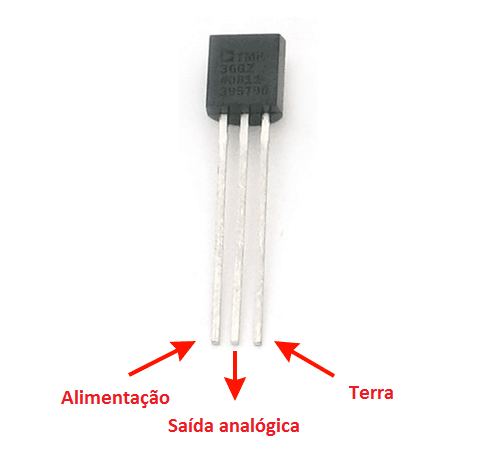
\includegraphics[width=10cm]{imagens/lm35.png}

\label{Sensor de temperatura}

\caption{Sensor de temperatura}

\end{figure}


O sensor possui três terminais: Alimentação, terra e saída analógica. O sensor pode ser alimentado com uma tensão contínua que varia de 4 à 30V e é capaz de medir temperaturas que variam de $-55\,^{\circ}{C}$ à $150\,^{\circ}{C}$. A precisão do sensor é de $ \pm 0,25\,^{\circ}{C}$ para medições de temperatura ambiente e de $ \pm 0,75\,^{\circ}{C}$ para medições entre $-55\,^{\circ}{C}$ à $150\,^{\circ}{C}$. A sua saída varia de 10mV para cada grau Celsius de temperatura, não havendo a necessidade de calibração (Datasheet LM35, 2013).
	
	O sensor possui baixa impedância de saída, tensão linear e calibração inerente precisa, tornando assim a interfaceamento de leitura de temperatura simples e barato (LM35 Datasheet, 2013).


\section{TRIAC}

O TRIAC (\textit{Triode for Alternating Current })  é um dispositivo de controle de corrente alternada. Ele é bastante semelhante ao SCR  (\textit{Silicon Controlled Rectifier}), porém ele possui a característica de conduzir corrente elétrica em dois sentidos. Ele é bastante utilizado quando há a necessidade de se controlar a potência aplicada a uma determinada carga elétrica. Ele é constituído por três terminais, MT1 (\textit{Main Terminal 1}), MT2 (\textit{Main Terminal 2}) e \textit{Gate}. A figura 2.8 representa o símbolo de um TRIAC bem como seus terminais.

\begin{figure}[h]

\center

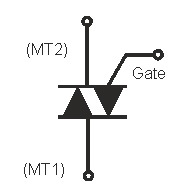
\includegraphics[width=4cm]{imagens/imagem_triac.jpg}

\label{TRIAC}

\caption{TRIAC}

\end{figure}

Um TRIAC pode ser disparado por uma tensão positiva ou negativa aplicada ao terminal de disparo (Gate), e a corrente normalmente na casa dos miliamperes. Ao ser disparado, o TRIAC conduz corrente elétrica até que este valor de corrente se reduza para um valor muito baixo (valor de corrente próximo a zero no final do ciclo de um sinal de corrente alternada). Dessa forma, o TRIAC se torna um componente de grande utilidade para correntes alternadas pois permite controlar altas potências a partir de circuitos acionados por correntes muito baixas.

O TRIAC também possibilita o controle de ângulo de fase de um sinal por simplesmente aplicar-se um pulso em um determinado instante do ciclo de corrente alternada. A figura 2.9 mostra o funcionamento do ângulo de fase.

\begin{figure}[h]

\center

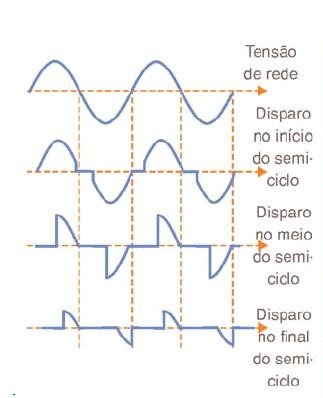
\includegraphics[width=7cm]{imagens/angulo_triac.jpg}

\label{Controle de ângulo de fase}

\caption{Controle de ângulo de fase}

\end{figure}
\noindent Quanto mais próximo do início do ciclo o disparo for dado, maior a potência será aplicada na carga.

\section{Optoacoplador}
O optoacoplador MOC 3020 é um dispositivo isolador que é constituído de um \textit{led} infravermelho e um fotodiac. Com este dispositivo se torna possível o controle de uma alta tensão a partir de uma baixa tensão. A figura 2.10 representa o símbolo de um optoacoplador.

\begin{figure}[h]

\center

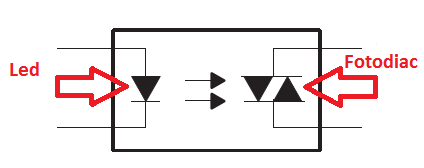
\includegraphics[width=10cm]{imagens/optoaco.png}

\label{Optoacoplador}

\caption{Optoacoplador}

\end{figure}

A corrente elétrica ao passar pelo LED infravermelho aciona um fotodiac do outro lado do circuito permitindo a passagem de corrente elétrica e dessa forma isolando o lado onde há uma alta tensão do lado onde se tem uma baixa tensão.




\section{Sistemas de controle}

Um sistema de controle é um método utilizado para controlar o comportamento de um determinado sistema onde a saída seja dependente da entrada. Um sistema pode ser interpretado como uma caixa preta com uma entrada e uma saída onde sabemos somente a relação entre elas (BOLTON, 1995). A figura 2.11 mostra a ilustração da interpretação de um sistema qualquer. 

\begin{figure}[!htb]

\center

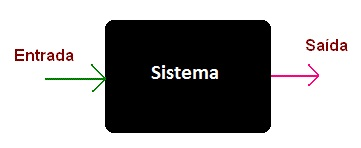
\includegraphics[width=7cm]{imagens/sistema_caixa_preta.jpg}

\label{Caixa preta}

\caption{Caixa preta}

\end{figure}

Para praticamente todos os tipos de sistemas é necessário um estudo de controle para que haja um funcionamento de acordo com o que se quer e seja alcançada a estabilidade do mesmo. Sem esse estudo o sistema pode funcionar de forma inadequada e nunca convergir para um determinado valor. A figura 2.12 mostra um gráfico como exemplo da estabilidade de um sistema em função do tempo, onde o \textit{set point}  é o valor que deseja-se na saída do sistema.


\begin{figure}[!htb]

\center

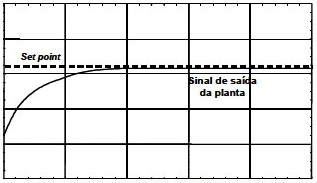
\includegraphics[width=10cm]{imagens/estabilidade_sistema.jpg}

\label{Estabilidade de um sistema}

\caption{Estabilidade de um sistema}

\end{figure}

A vantagem de se estudar sistemas de controle é que inúmeros sistemas com propriedades completamente diferentes podem ter a mesma relação de entrada e saída, como por exemplo a resposta de um capacitor em série com um resistor a uma determinada tensão. Este sistema tem o mesmo tipo de relação com um recipiente cheio de um liquido do qual é aplicado uma determinada entrada de calor (BOLTON, 1995). 

\subsection{Transformada de Laplace}

Uma ferramenta matemática bastante útil no estudo de sistemas de controle é a transformada de Laplace. Esta ferramenta tem o poder de transformar equações diferenciais em equações algébricas das quais são mais facilmente solucionáveis. Operações como integrais e derivadas podem ser substituídas por equações algébricas no plano complexo.  Quando aplica-se a transformada de Laplace a um sistema ele sai do domínio do tempo e passa a ser analisado no domínio $s$ (domínio da frequência complexa)  (BOLTON, 1995). Além de facilitar bastante os cálculos, a análise neste domínio nos fornece informações sobre o comportamento do sistemas em regime transitório (antes de estabilizar) e em regime permanente (após estabilizar).

A transformada de Laplace é aplicada da seguinte forma: multiplica-se cada termo na equação por $e^{-sT}$, onde $s$ é uma  constante com unidade $ \frac {1}{tempo}$  e então integrar cada termo em relação ao tempo de zero até infinito. O resultado é o que chama-se de transformada de Laplace. Portanto, a transformada de Laplace de algum termo, que é função do tempo, é:

\begin{center} 
$F(s) = \int_0^\infty f(t) e^{-sT} dt,$
\end{center}

onde $f(t)$ é uma função no domínio do tempo e $F(s)$ é a transformada de Laplace desse termo no domínio de $s$ (BOLTON, 1995).

\subsection{Sistemas de controle em malha aberta}

Os sistemas de controle em malha aberta são sistemas onde a saída não influencia no controle do sistema, ou seja, não é verificado um erro da resposta em relação a entrada. Um exemplo disso seria a máquina de lavar roupas. A máquina não verifica se a roupa está bem limpa no final da lavagem, ela apenas executa suas funções em sequência em um determinado tempo. Logo, não temos uma verificação do sinal de saída (roupa limpa) por um sinal de entrada (roupa limpa) (OGATA, 2003). A figura 2.13 mostra o sistema de controle em malha aberta de uma máquina de lavar roupas.

\begin{figure}[!htb]

\center

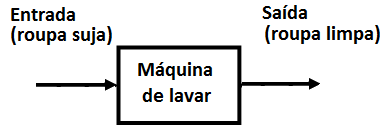
\includegraphics[width=10cm]{imagens/malha_aberta.png}

\label{Sistema em malha aberta}

\caption{Sistema em malha aberta}

\end{figure}


Este tipo de sistema de controle é normalmente utilizado quando se tem um conhecimento da relação entre a entrada e a saída do sistema e também com a ausência de possíveis distúrbios internos ou externos. O sistema de controle em malha aberta apresenta, normalmente, um erro em regime permanente, ou seja, um erro quando o sistema já está estabilizado.

\subsection{Sistemas de controle em malha fechada}

Os sistemas de controle em malha fechada são sistemas onde a saída influencia no controle do mesmo. O erro (a diferença entre o valor de saída e o valor de entrada) excita o controlador para que este erro seja eliminado ou minimizado na próxima iteração(OGATA, 2003). Este é um sistema de controle utilizado em vários aparelhos, como por exemplo uma geladeira onde a temperatura é constantemente medida para que quando atinja um certo valor ela se desligue, economizando assim energia elétrica.A figura 2.14 um exemplo de sistema de controle em malha fechada do funcionamento de uma geladeira.

\begin{figure}[H]

\center

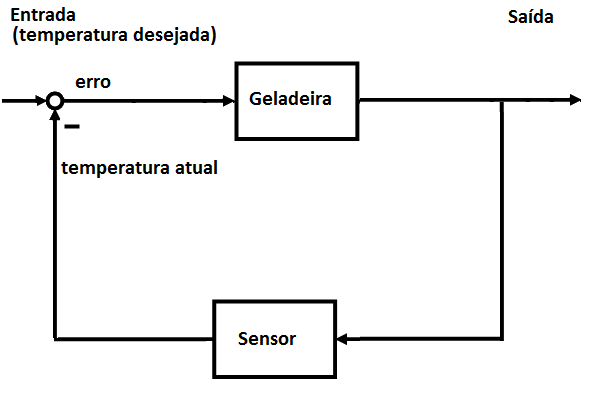
\includegraphics[width=12cm]{imagens/malha_fechada.png}

\label{Sistema em malha fechada}

\caption{Sistema em malha fechada}

\end{figure}


\subsection{Comparação entre os tipos de sistemas de controle}

A principal vantagem de um sistema de controle em malha fechada é a possível correção do erro do sistema o que o torna mais estável quando há perturbações externas ou internas. É possível a utilização de componentes baratos, sem muita exatidão para se conseguir um controle preciso de um determinado processo, fato que se torna impossível na utilização de um sistema de controle em malha aberta. Mas em relação a estabilidade de um sistema, os controles em malha aberta são, normalmente, mais fáceis de serem implementados, pois o controle em malha fechada pode tender a corrigir erros além do necessário ocasionando uma oscilação com amplitude constante ou cada vez maior com o passar do tempo(OGATA, 2003).

\subsection{Controladores}
Os controladores são estratégias utilizadas para se fazer com que um sistema físico atenda as especificações de funcionamento e desempenho determinadas.  Basicamente um controlador é um elemento no sistema de controle em malha fechada que tem como entrada o erro do sistema e gera uma saída que se torna a entrada para a planta do sistema (BOLTON, 1995). A figura 2.15 mostra um exemplo de planta realimentada com utilização de um controlador.

\begin{figure}[!htb]

\center

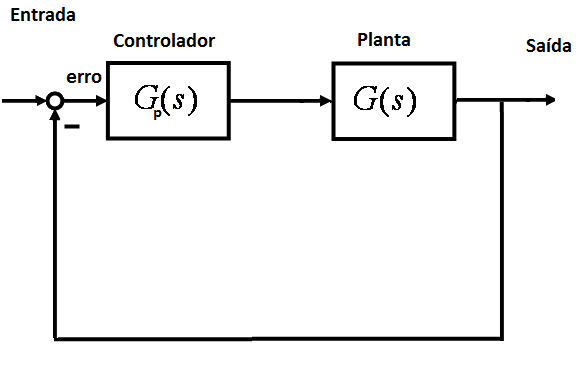
\includegraphics[width=12cm]{imagens/planta_realimentada.png}

\label{Planta realimentada com controlador}

\caption{Planta realimentada com controlador}

\end{figure}

Existem três formas principais de se implementar um controlador que utiliza o parâmetro de erro entre a referência e a saída: proporcional, integral e derivativa.

\subsection{Controlador proporcional}

Um controlador proporcional tem a relação de entrada $e(t)$ e saída $u(t)$ da seguinte forma:

\begin{center}
$u(t) = K_p.e(t)$
\end{center}

\noindent onde pode-se notar que o sinal de saída do controlador é proporcional ao erro do sistema. Passando para o domínio de $s$ com a transformada de Laplace obtemos a função de transferência:

\begin{center}
$\frac {U(s)}{E(s)} = K_p$
\end{center}

\noindent onde $Kp$ é denomidado o ganho proporcional.

Independente do mecanismo, o controlador proporcional nada mais é do que um amplificador com um ganho ajustável. A figura 2.16 representa o diagrama de blocos de um controlador proporcional (OGATA, 2003).

\begin{figure}[H]

\center

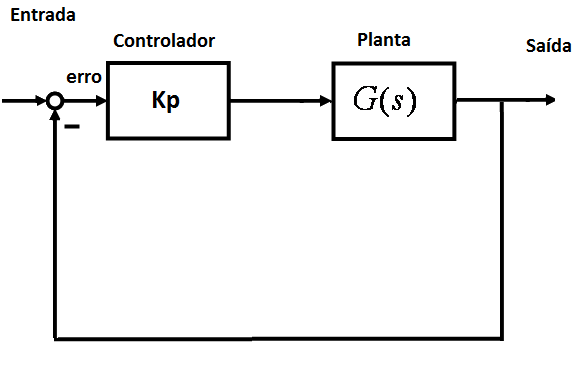
\includegraphics[width=10cm]{imagens/planta_proporcional.png}

\label{Diagrama de blocos do controlador proporcional}

\caption{Diagrama de blocos do controlador proporcional}

\end{figure}

\subsection{Controlador Integral}
A relação de entrada e saída de um controlador integral é dada pela seguinte equação:

\begin{center}
$ u(t) = K_i \int_0^t e(t)dt$
\end{center}

\noindent onde $Ki$ é uma constante denominada de ganho integral. A função de transferência de um controlador integral é dada pela equação abaixo:

\begin{center}
$ \frac{U(s)}{E(s)} = \frac{K_i}{s}$
\end{center}

\noindent Desta forma, a saída em qualquer instante de tempo é proporcional ao acúmulo de efeitos do erro em instantes anteriores (BOLTON, 1995). A figura 2.17 mostra um diagrama do controlador integral.


\begin{figure}[!htb]

\center

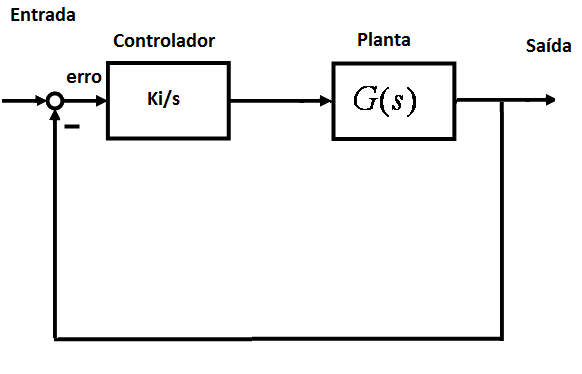
\includegraphics[width=10cm]{imagens/planta_integral.png}

\label{Diagrama de blocos do controlador integral}

\caption{Diagrama de blocos do controlador integral}

\end{figure}

\subsection{Controlador Derivativo}

A saída de um controlador derivativo é proporcional à taxa de variação do erro, $e(t)$, ou seja:

\begin{center}
$u(t) = K_d \frac{d e(t)}{dt}$

\end{center}
\noindent onde $K_d$ é denominado de ganho derivativo.

A função de transferência do controlador derivativo é definida por:

\begin{center}
$\frac{U(s)}{E(s)} = K_d.s$

\end{center}

Com  o controlador derivativo, quando há sinal de erro a saída do controlador já torna-se grande pois ele é proporcional a taxa de variação do sinal de erro e não do erro em si. Isso fornece uma grande correção no erro, entretanto se o erro for um valor constante nenhuma ação será executada pelo controlador (BOLTON, 1995). A figura 2.18  mostra o diagrama de blocos de um controlador derivativo.

\begin{figure}[!htb]

\center

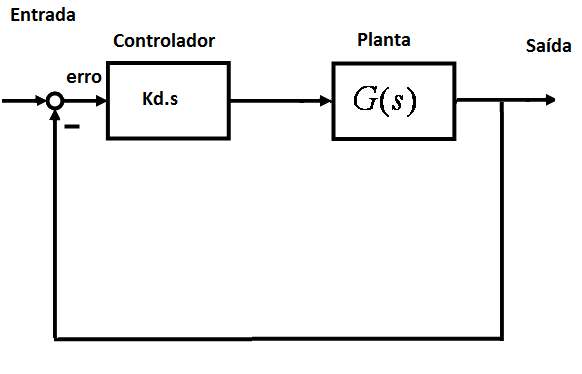
\includegraphics[width=10cm]{imagens/planta_derivativo.png}

\label{Diagrama de blocos do controlador derivativo}

\caption{Diagrama de blocos do controlador derivativo}

\end{figure}

\subsection{Preditor de Smith}

Normalmente, em diversos tipos de processos há a presença de um \textit{delay}, ou seja, um determinado tempo de atraso para um processo sentir a variação da entrada na saída. Em sistemas de controle este \textit{delay} é denominado tempo morto e ele existe sempre que há transporte físico de energia ou material. Um exemplo da presença de tempo morto é mostrado na figura 2.19.

\begin{figure}[H]

\center

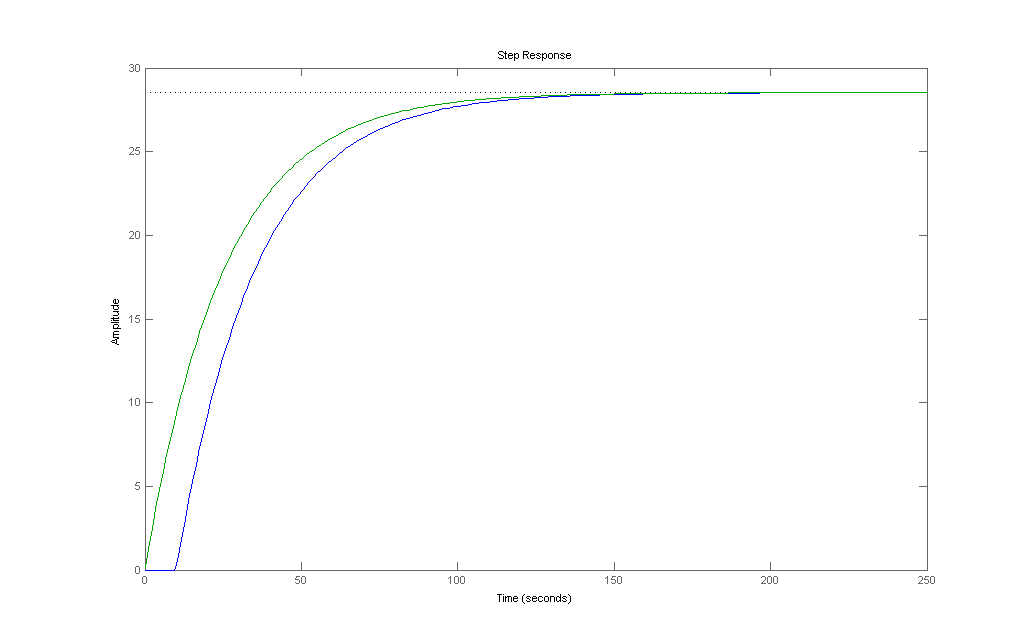
\includegraphics[width=12cm]{imagens/tempo_morto.png}

\label{Tempo morto}

\caption{Tempo morto}

\end{figure}

Pode-se ver que o sistema (linha azul) demorou um certo tempo para a responder a entrada (linha verde)

Quando há a presença de tempo morto em algum tipo de processo há também uma diminuição no desempenho do 
sistema de controle por realimentação. O ganho controlador tem que ser reduzido em relação ao sistema de controle utilizado caso o sistema não tivesse tempo morto (MACHADO, 2004).

Para driblar esse problema presente em inúmeras aplicações na engenharia, processos industriais, entre muitos outros,  O. J. M. Smith (SMITH, 1959) propôs um esquema de controle bastante poderoso  para melhorar a eficiência de malhas de controle com presença de tempo morto. Este esquema de controle ficou conhecido como Preditor de Smith. O Preditor de Smith utiliza um sistema de realimentação interna em malha fechada que elimina o tempo morto do sistema a ser controlado. A figura 2.20 representa o diagrama de blocos de um Preditor de Smith.

\begin{figure}[!htb]

\center

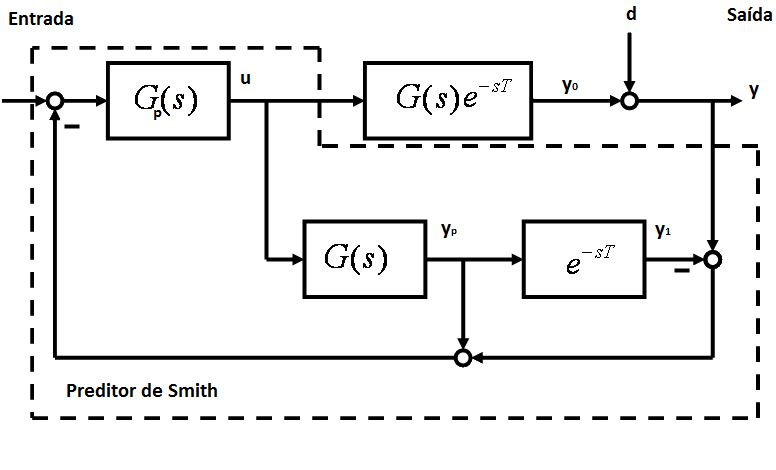
\includegraphics[width=10cm]{imagens/Preditor_de_smith.png}

\label{Preditor de Smith}

\caption{Preditor de Smith}

\end{figure}

Na figura acima, $G(s)$ é a planta do sistema, $e^{-sT}$ é o atraso do sistema,$G_p(s)$ representa o controlador e $d$ representa um possível distúrbio externo. A equação abaixo mostra a função de transferência resultante da malha fechada.

\begin{center}

$\frac{SAIDA}{ENTRADA} = \frac{G_p(s).G(s).e^{-sT}}{1+ G_p(s).G(s)}$

\end{center}

Dessa maneira consegue-se eliminar o tempo de atraso $e^{-sT}$ da equação característica do sistema e portanto tem-se uma melhora significante no controle do mesmo. Após aplicado o esquema do Preditor de Smith, podemos redesenhar o diagrama de blocos como mostra a figura 2.21.

\begin{figure}[!htb]

\center

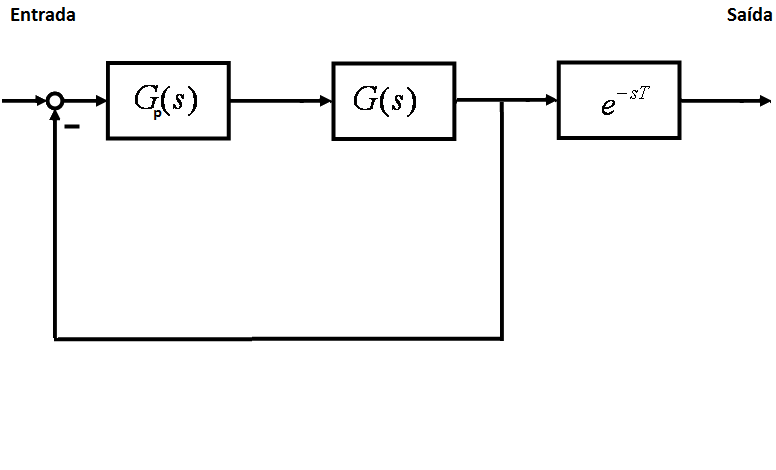
\includegraphics[width=10cm]{imagens/Preditor_de_smith_equivalente.png}

\label{Diagrama de blocos equivalente}

\caption{Diagrama de blocos equivalente}

\end{figure}

Pode-se notar que o diagrama de blocos equivalente do Preditor de Smith coloca o tempo morto para fora da malha fechada o que não afetará a performance dinâmica do controlador.

\section{Matlab}

O \textit{MathWorks} Matlab é um software poderoso destinado à manipulação de matrizes, plotagem de funções, implementação de algoritmos, dentre outros. É considerada uma linguagem de alto nível e possui um ambiente para cálculos, visualização e programação computacional (Matlab, 2013). O Matlab abrange uma gama grande de aplicações como processamentos de sinais, processamento  de vídeo e imagens, biologia, economia, entre outros.

Neste trabalho, o Matlab  foi utilizado para  a obtenção do modelo da planta, simulação da planta e dos controladores, e projeto dos controladores. 
\chapter{Desenvolvimento}

Esse capítulo irá discorrer sobre as metodologias e procedimentos utilizados no desenvolvimento da ferramenta.

\chapter{Resultados}

Três testes com diferentes temperaturas de referência foram realizados para que fosse possível a análise da eficiência do regulador. Nos três testes, a temperatura ambiente encontrava-se por volta de 27$^{\circ}$C. Os dados de temperatura foram adquiridos utilizando-se o próprio sensor LM35.

    O primeiro teste foi realizado com a referência (temperatura desejada da água) para 34$^{\circ}$C. A figura 5.1 mostra o gráfico da temperatura da água em função do tempo.
    
\begin{figure}[H]

\center

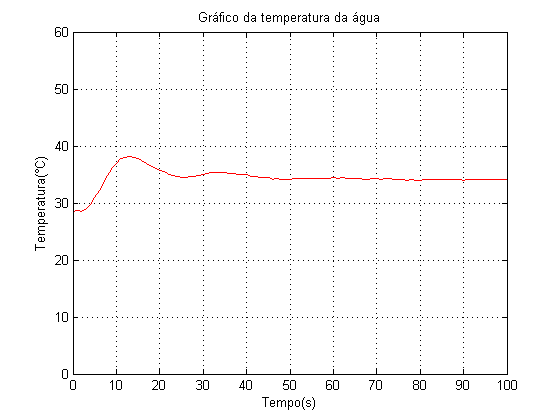
\includegraphics[width=10cm]{imagens/grafico_34graus.png}

\label{Temperatura da água para referência em 34 graus Celsius}

\caption{Temperatura da água para referência em 34 graus Celsius}
\end{figure}
    
\noindent É possível notar uma pequena variação na temperatura após o sistema atingir o regime permanente (cerca de 40 segundos). Essa variação, apesar de não influenciar de forma relevante na variação da temperatura, provavelmente se dá devido ao ruído do sensor LM35. 

    Mesmo com a presença de ruídos no sensor de temperatura, o regulador teve uma eficiência satisfatória, com baixíssimas variações em relação a temperatura desejada, que dificilmente seriam notadas na pele de uma pessoa.

O segundo teste realizado foi para a temperatura desejada de 37$^{\circ}$C. A figura 5.2 mostra o gráfico para o teste realizado.
\begin{figure}[H]
\center

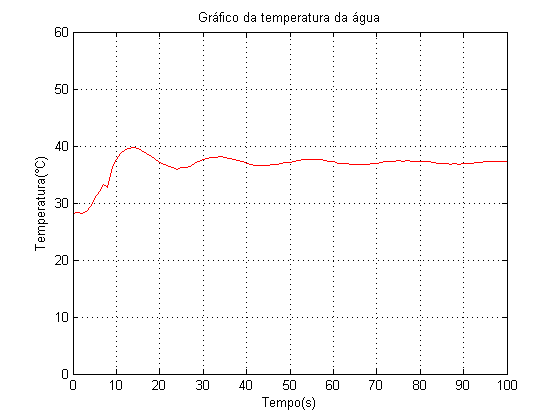
\includegraphics[width=10cm]{imagens/grafico_37graus.png}

\label{Temperatura da água para referência em 37 graus Celsius}

\caption{Temperatura da água para referência em 37 graus Celsius}
\end{figure}

\noindent Neste caso pode-se perceber que o ruído no sensor teve uma influência maior, pois após o tempo de regime permanente as variações foram um pouco maiores que as analisadas no primeiro teste, porém, como o primeiro teste, essas variações seriam dificilmente notadas em um banho.

O terceiro e último teste foi realizado com a temperatura desejada de 40$^{\circ}$C. A figura 5.3 mostra o gráfico para o último teste.
\begin{figure}[H]
\center

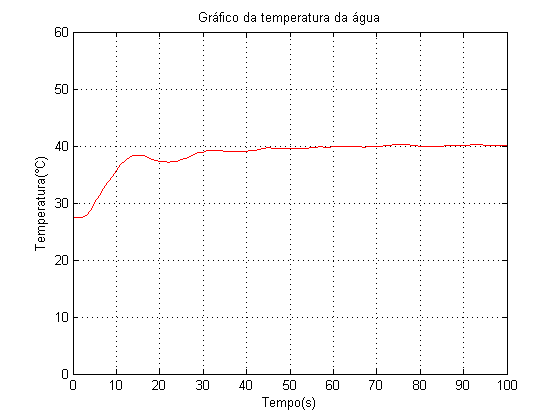
\includegraphics[width=10cm]{imagens/grafico_40graus.png}

\label{Temperatura da água para referência em 40 graus Celsius}

\caption{Temperatura da água para referência em 40 graus Celsius}
\end{figure}

\noindent O comportamento deste teste foi bastante semelhante ao do primeiro. As variações de temperatura após a estabilização foram baixíssimas, em torno de 0,2$^{\circ}$C à 0,3$^{\circ}$C.

Com base nos gráficos apresentados para os testes, pode-se notar que o regulador de temperaturas funciona de forma satisfatória com erros que variam em torno de  0,2$^{\circ}$C à 0,3$^{\circ}$C, valores que a pele humana dificilmente irá sentir em um banho. O tempo de ajuste de temperatura da água do banho foi reduzido de dois minutos (tempo médio para ajuste da temperatura ideal de um chuveiro convencional) para cerca de 40 segundos.
\chapter{Conclusão}

O código-fonte de ferramenta será futuramente disponibilizado, sob licença de software livre, para permitir que seu desenvolvimento seja continuado.

\section{Futuras melhorias}


\begin{thebibliography}{99}
\bibitem{aniche} ANICHE, M. \textbf{Test-Driven Development}. Disponível em \url{http://tdd.caelum.com.br/}. Acesso em 19 mai. 2015.

\bibitem{an738} \textbf{Application Note 738: Minimizing Component-Variation Sensitivity in
Single Op Amp Filters}. Disponível em \url{http://pdfserv.maximintegrated.com/en/an/AN738.pdf}. Acesso em 15 jun. 2015.

\bibitem{an1762} \textbf{Application Note 1762: A Beginner's Guide to Filter Topologies}. Disponível em \url{http://pdfserv.maximintegrated.com/en/an/AN1762.pdf}. Acesso em 01 abr. 2015.

\bibitem{barros} BARROS, A. M. \textbf{Projeto de Filtros FIR através de Algoritmos Genéticos}. Dissertação (Mestrado em Engenharia Elétrica e Informática) - Universidade Tecnológica Federal do Paraná. Curitiba, 2006. % http://files.dirppg.ct.utfpr.edu.br/cpgei/Ano_2006/dissertacoes/Dissertacao_400_2006.pdf

\bibitem{butterworth} BUTTERWORTH, S. \textbf{On the Theory of Filter Amplifiers}. \textit{Wireless Engineer}, v. 7, p 536-541, 1930. 

\bibitem{tdd} CARDOSO, A. \textbf{TDD, por que usar?}. Disponível em \url{http://www.devmedia.com.br/tdd-fundamentos-do-desenvolvimento-orientado-a-testes/28151}. Acesso em 22 abr. 2015.

\bibitem{dattorro} DATTORRO, J. \textbf{The Implementation of Recursive Digital Filters for High-Fidelity Audio}. \textit{Journal of the Audio Engineering Society}, v. 36, n. 11, p. 851-878, 1988.

\bibitem{ti_dsp} \textbf{Digital Signal Processors - Texas Instruments}. Disponível em \url{http://www.ti.com/DSP}. Acesso em 15 abr. 2015.

\bibitem{diniz} DINIZ, P. S. SILVA, E. A. B. NETTO, S. L. \textbf{Processamento digital de sinais: projeto e análise de sistemas}. 2\textsuperscript{a} edição. Porto Alegre: Bookman, 2014. 1000p.

\bibitem{dspic} \textbf{dsPIC30F Programmer's Reference Manual}. Disponível em \url{http://ww1.microchip.com/downloads/en/DeviceDoc/sect3_4.pdf}. Acesso em 15 abr. 2015.

\bibitem{filterlab} \textbf{FilterLab Filter Design software.} Disponível em \url{http://www.microchip.com/pagehandler/en_us/devtools/filterlab-filter-design-software.html}. Acesso em 22 abr. 2015.

\bibitem{fortunato} FORTUNATO, M. \textbf{Circuit Sensitivity With Emphasis On Analog Filters}. Disponível em \url{http://www.ti.com/lit/ml/sprp524/sprp524.pdf}. Acesso em 15 jun. 2015.

\bibitem{analog} \textbf{Filter Wizard}. Disponível em \url{http://www.analog.com/designtools/en/filterwizard/#/specifications}. Acesso em 11 jun. 2015.

\bibitem{harris} HARRIS, F, J. \textbf{On the use of windows for harmonic analysis with the discrete Fourier transform}. \textit{Proceedings of the IEEE}, v. 66, n. 1, p. 51-83, 1978.

\bibitem{haykin} HAYKIN, S. VAN VEEN, B. \textbf{Sinais e Sistemas}. 1\textsuperscript{a} edição. Porto Alegre: Bookman, 2001. 661 p.

\bibitem{horowitz} HOROWITZ, P. HILL, W. \textbf{The Art of Electronics}. 2\textsuperscript{a} edição. Cambridge: Cambridge University Press, 1989. 1125p.

\bibitem{jung} JUNG, W. \textbf{Op Amp Applications Handbook.} Disponível em \url{http://www.analog.com/library/analogDialogue/archives/39-05/op_amp_applications_handbook.html}. Acesso em 18 jun. 2015.

\bibitem{khn} KERWIN, W. J. HUELSMAN, L. P., NEWCOMB, R. W. \textbf{State Variable Synthesis for Insensitive Integrated Circuit Transfer Functions}. \textit{IEEE Journal of Solid-State Circuits}, v. SC-2, n. 3, p. 87-92, 1967.

\bibitem{mancini} MANCINI, R. et al. \textbf{Op-Amps for Everyone}. 4\textsuperscript{a}  edição. Burlington: Newnes, 2003. 304p.

\bibitem{marques} MARQUES, A. A. de A. \textbf{Projeto e implementação em tempo real de filtros digitais utilizando microprocessadores de sinal}. 1996. 201p. Dissertação (Mestrado em Engenharia Eletrotécnica e de Computadores) - Faculdade de Engenharia da Universidade do Porto. Porto, 1996. % http://repositorio-aberto.up.pt/bitstream/10216/12788/2/%20Texto%20integral.pdf

\bibitem{mcclellan} MCCLELLAN, J. PARKS, T. \textbf{A unified approach to the design of optimum FIR linear-phase digital filters}. \textit{IEEE Transactions on Circuit Theory}, v. 20, n. 6, p. 697-701, 1973.

\bibitem{mcclellan_2} MCCLELLAN, J. PARKS, T. RABINER, L. \textbf{A Computer Program for Designing Optimum FIR Phase Digital Filters}. \textit{IEEE Transactions on Audio and Electroacoustics}, v. AU-21, n. 6, p. 506-526, 1973.

\bibitem{numpydoc} NumPy and SciPy documentation. Disponível em \url{http://docs.scipy.org/doc/}. Acesso em 22 mar. 2015.

\bibitem{oppenheim} OPPENHEIM, A. V. WILLSKY, A.S. \textbf{Sinais e Sistemas}. 2\textsuperscript{a} edição. São Paulo: Pearson Prentice-Hall, 2010. 568p.

\bibitem{orfanidis} ORFANIDIS, S. J. \textbf{Lecture Notes on Elliptic Filter Design}. Disponível em \url{http://eceweb1.rutgers.edu/~orfanidi/ece521/notes.pdf}. Acesso em 13 mai. 2015.

\bibitem{paarmann} PAARMANN, L. D. \textbf{Design and Analysis of Analog Filters: A Signal Processing Perspective}. New York: Kluwer Academic Publishers, 2003. 453p.

\bibitem{pythondoc} Python 3.4.3 Documentation. Disponível em \url{https://docs.python.org/3/}. Acesso em 03 mar. 2015.

\bibitem{quelhas} QUÉLHAS, M. F. \textbf{Projeto de Filtros IIR por Mapeamento de Polos e Zeros}. 2010. 132p. Tese (Doutorado em Engenharia Elétrica) - COPPE, Universidade Federal do Rio de Janeiro. Rio de Janeiro, 2010. % http://www.pee.ufrj.br/teses/textocompleto/2010080601.pdf

\bibitem{razavi} RAZAVI, B. \textbf{Fundamentos de Microeletrônica}. 1\textsuperscript{a} edição. Rio de Janeiro: LTC, 2013. 728p.

\bibitem{rowell} ROWELL, D. \textbf{Signal Processing: Continuous and Discrete}. Disponível em \url{http://ocw.mit.edu/courses/mechanical-engineering/2-161-signal-processing-continuous-and-discrete-fall-2008/lecture-notes/}. Acesso em 13 mai. 2015.

\bibitem{sallen} SALLEN, R. P. KEY, E. L. \textbf{A  Practical Method of Designing RC Active Filters}. \textit{IRE Transactions on  Circuit Theory}, v. 2, n. 1, p. 74-85, 1955.

\bibitem{sancho} SANCHOTENE, R. RODRIGUES, C. R. \textbf{A 120s-time-constant 2$^{nd}$ order Butterworth low-pass Gm-C filter based on a novel Reverse Cascode topology}. EMICRO 2015, Santa Maria, 2015. % Verificar a citação

\bibitem{sedra_smith} SEDRA, A. S. SMITH, K. C. \textbf{Microeletrônica}. 5\textsuperscript{a} edição. São Paulo: Pearson Prentice-Hall, 2007. 848p.

\bibitem{souza} SOUZA, A. A. V. B. \textbf{Análise de Operadores Explícitos de Migração no Domínio $\omega - x$}. 2010. 60f. Trabalho de Conclusão de Curso (Graduação em Geofísica) - Instituto de Geociências, Universidade Federal da Bahia, Salvador, 2000. % http://www.cpgg.ufba.br/gr-geof/geo213/trabalhos-graducao/Alan-Souza.pdf

\bibitem{smith_dsp} SMITH, S. \textbf{The Scientist and Engineer's Guide to Digital Signal Processing}. 1\textsuperscript{a}  edição. s.l: California Technical Publishers, 1997. 626p. Disponível em \url{http://www.dspguide.com/}. Acesso em 11 mar. 2015.

\bibitem{sympydoc} SymPy Documentation. Disponível em \url{http://docs.sympy.org/latest/index.html}. Acesso em 25 mai. 2015.

\bibitem{an727} \textbf{TUTORIAL 727: Filter Design Using Integrator Blocks}. Disponível em \url{http://pdfserv.maximintegrated.com/en/an/AN727.pdf}. Acesso em 15 jun. 2015.



\bibitem{uaf42} \textbf{UAF42: Universal Active Filter}. Disponível em \url{http://www.ti.com/lit/ds/symlink/uaf42.pdf}. Acesso em 01 abr. 2015.

\bibitem{ti_filter} \textbf{WEBENCH Filter Designer}. Disponível em \url{http://www.ti.com/lsds/ti/analog/webench/webench-filters.page}. Acesso em 22 abr. 2015.

\bibitem{zumbalen} ZUMBALEN, H. \textbf{Linear Circuit Design Handbook}. 1\textsuperscript{a} edição. Burlington: Newnes, 2008. 960p. % http://www.analog.com/library/analogDialogue/archives/43-09/linear_circuit_design_handbook.html
\end{thebibliography}

\setlength{\baselineskip}{\baselineskip}

%%=============================================================================
%% Referências
%%=============================================================================
%\bibliographystyle{abnt}
%\bibliography{referencias/referencias}



%IMPORTANTE: Se precisar usar alguma seção ou subseção dentro dos apêndices ou
%anexos, utilizar o comando \tocless para não adicionar no Sumário
%Exemplos: 
% \tocless\section{Histórico}
%%=============================================================================
%% Apêndices
%%=============================================================================
%\appendix
%
\chapter{Título do apêndice}
Este é o apêndice A

%IMPORTANTE: Se precisar usar alguma seção ou subseção dentro dos apêndices ou
%anexos, utilizar o comando \tocless para não adicionar no Sumário
%Exemplos: 
% \tocless\section{Histórico}
% \tocless\subsection{Detalhes}
\tocless\section{teste}
Este é um teste de seção dentro do apêndice


%
\chapter{Título do apêndice Ex}
Esta é o apêndice B




\end{document}
